\chapter{Case study}
\label{chapter:case_studies}

This case-study explores the tradeoff of different skipping microarchitectures in a scenario where the sparse tensor accelerator exploits a SIMD MAC.

\section{Methodology}

 Here one case study is provided which showcases

\begin{itemize}
    \item SAF microarchitecture taxonomic inference with SAFinfer.
    \item SAF microarchitecture scale inference with SAFmodel.
    \item Tradeoff study comparing different choices of coordinate-payload intersection unit.
\end{itemize}

SAFmodel was also used to generate Accelergy analytical models for use with Sparseloop; however, for a variety of reasons, these models were not integrated into a Sparseloop testbench; the tradeoff study here only compares the energy-per-action and area overhead of SAF microarchitectures but does not use Sparseloop to obtain action counts or get energy/area estimates for the rest of the architecture.

SAFTools allows the user to customize the objective function for optimizing SAF microarchitecture. In this work, the objective function is the total energy-per-action/area product, over all SAF microarchitecture primitives and all actions. This is the default SAFTools objective function, and it is chosen in order to co-optimize energy and area. 

\begin{figure}[ht]
\centering
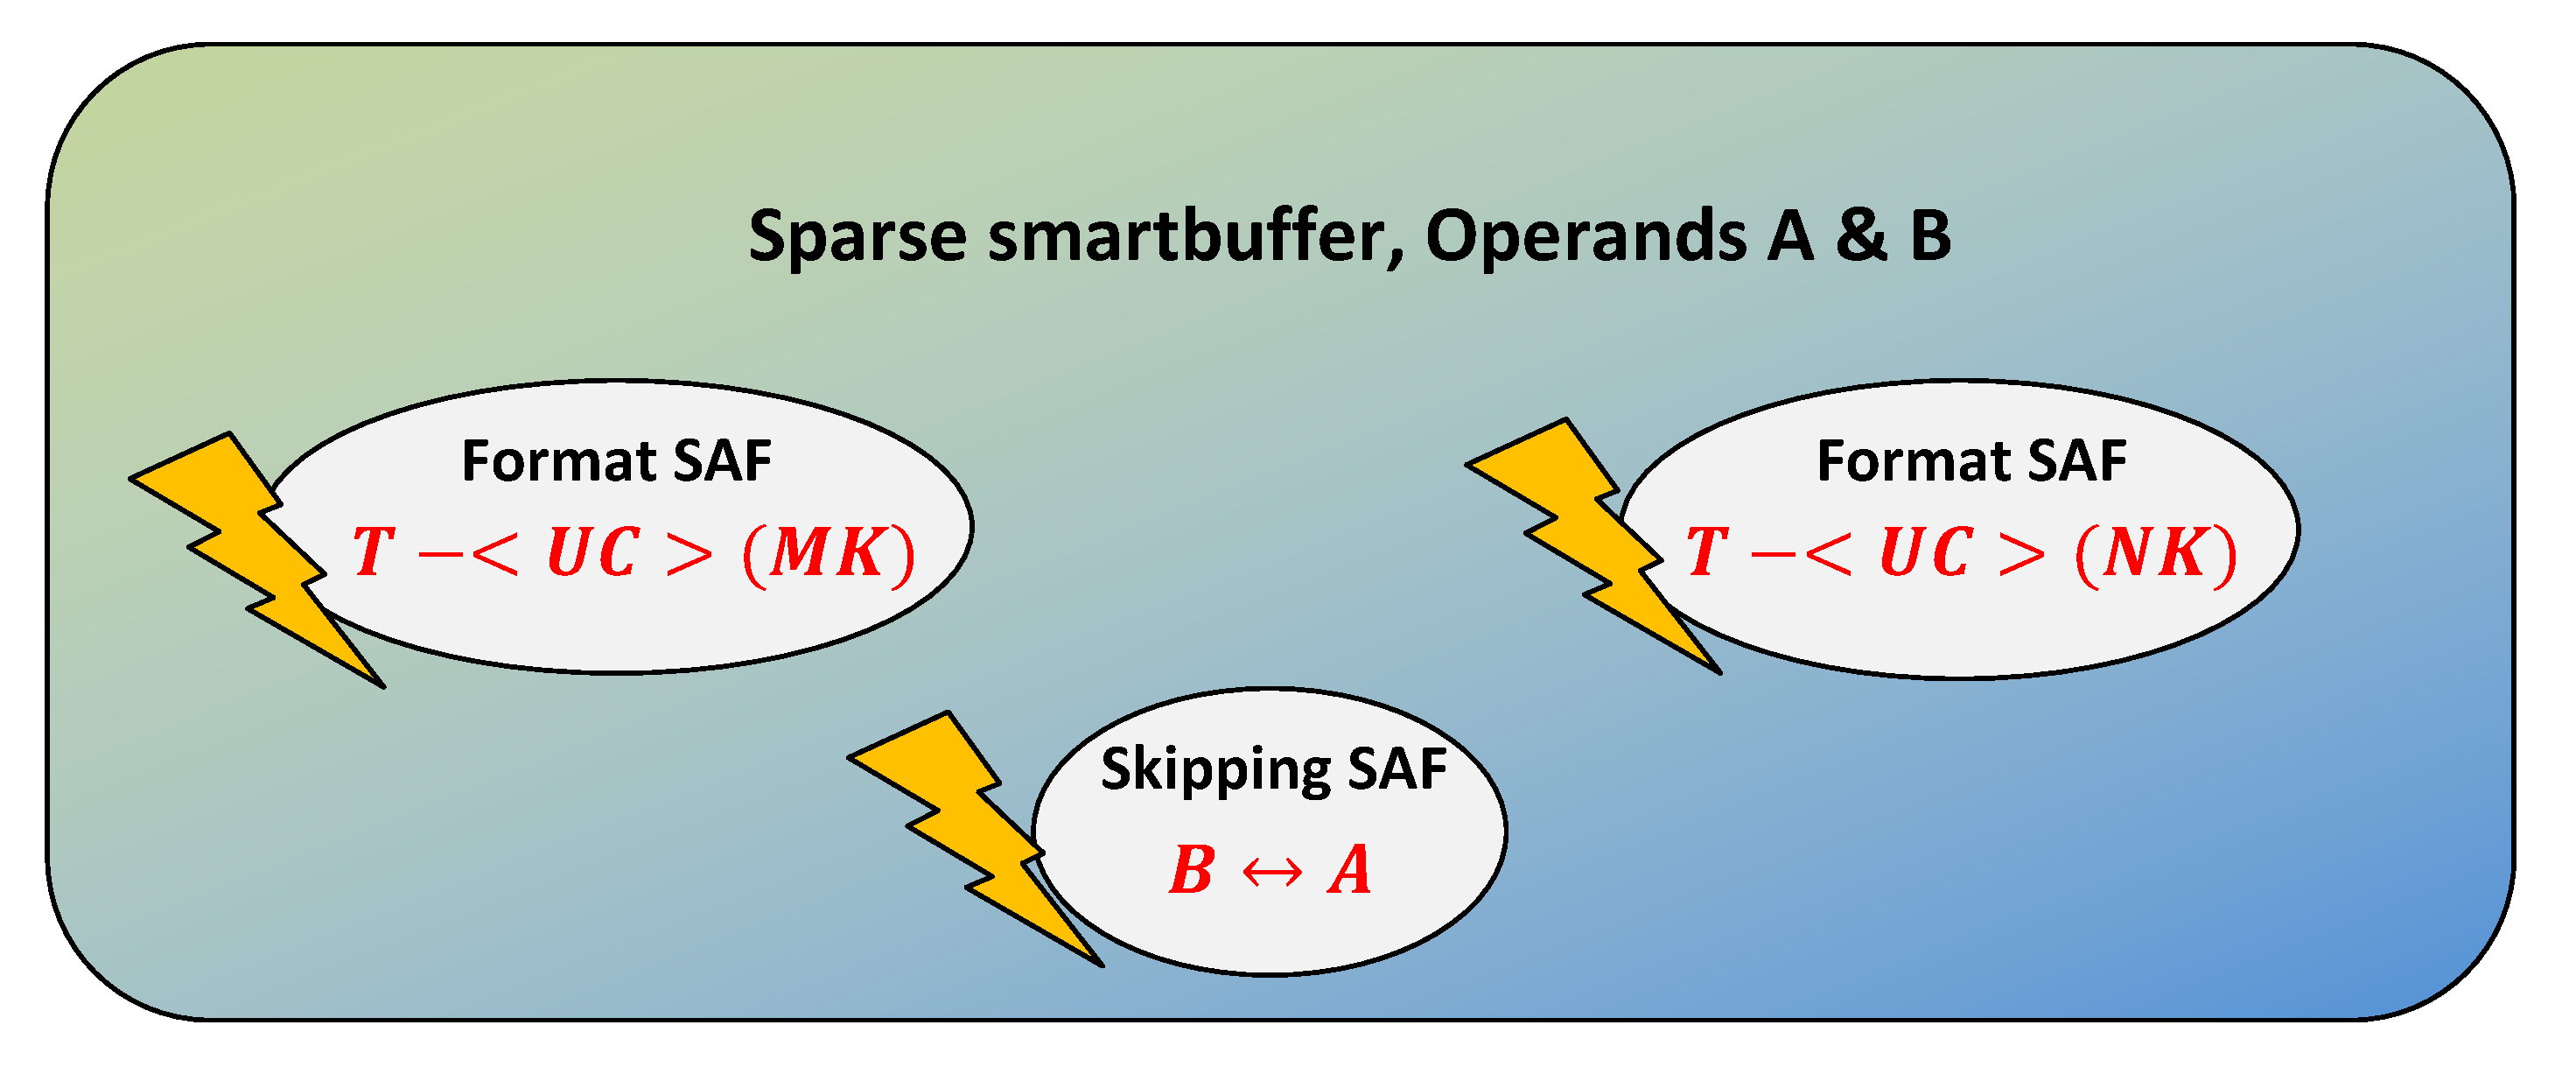
\includegraphics[width=0.85\textwidth]{figures/case_study_declarative.pdf}
\caption{Sparseloop configuration files provided to SAFinfer.}
\label{fig:case_study_declarative}
\end{figure}

For taxonomic inference, SAFinfer was provided Sparseloop configuration files specifying a hypothetical architecture with a buffer holding both input operands resident, both in CSR format (T-<UC>(MK) and T-<UC>(NK) respectively), and subject to a bidirectional skipping SAF. This state of affairs is summarized in Figure~\ref{fig:case_study_declarative}. This Sparseloop configuration file is meant to represent spGEMM without tiling\footnote{SAFinfer only consumes the Sparseloop architecture and Sparseopts files; SAFinfer does not have access to the problem einsum or mapping\cite{sparseloop}.} Additionally there is a single partial sum register for accumulating the inner product in a dense/uncompressed format.

For scale inference, SAFmodel was provided the SAFinfer output microarchitecture as well as a requirement to use energy-per-action/area product as the objective function to minimize during scale inference. SAFmodel was instrumented to output a sweep over valid scale parameter configurations $\{S_x\}_{valid}$, for the purposes of visualizing and comparing possible combinations of low-level scale parameters such as input vectorization, pipeline depth, etc.

Designs such as Eyeriss v2\cite{eyerissv2} exploit SIMD MAC units in order to accelerate processing, however this places increased pressure on the rest of the design to support doubled throughput. This observation suggested an opportunity to explore the impact of throughput requirements on scale inference in skipping microarchitectures.

\section{Results}

\subsection{Inferred SAF microarchitecture}

\begin{figure}[ht]
\centering
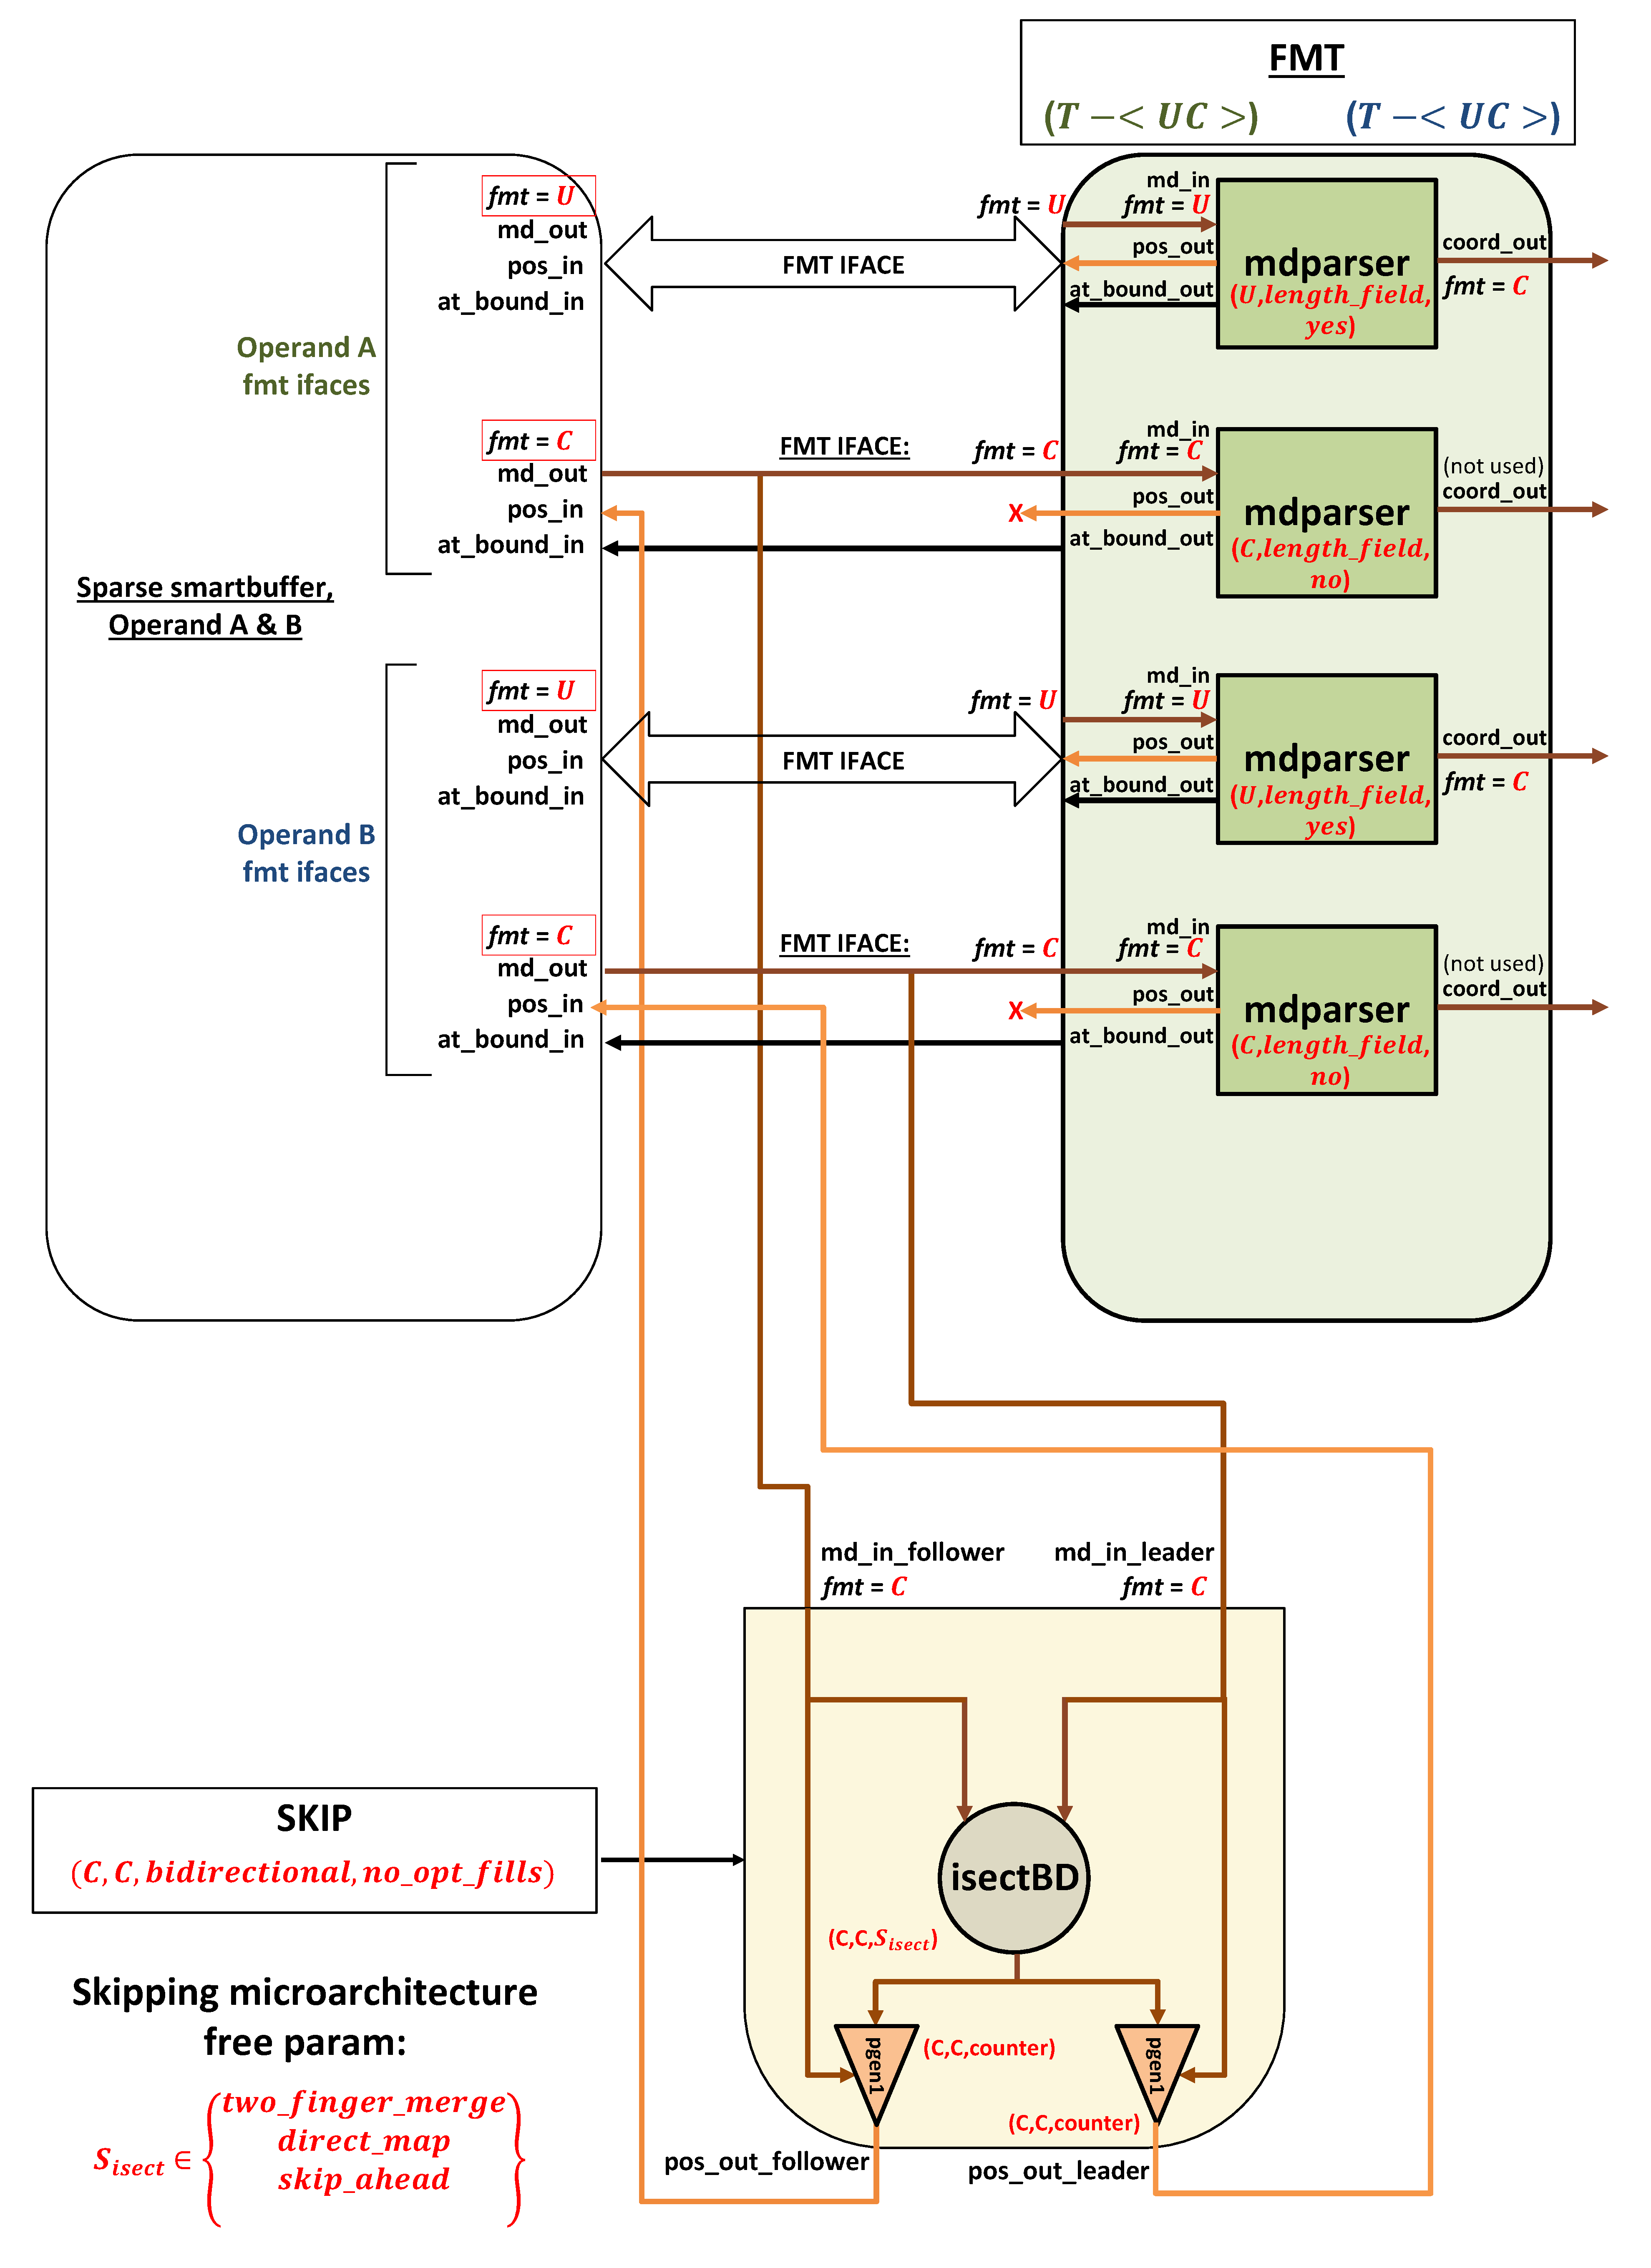
\includegraphics[width=0.7\textwidth]{figures/case_study_inferred_uarch.pdf}
\caption{SAF microarchitecture synthesized by SAFinfer based on declarative specifications.}
\label{fig:case_study_inferred_uarch}
\end{figure}

\clearpage

Figure~\ref{fig:case_study_inferred_uarch} shows the SAF microarchitecture inferred by SAFinfer based on the declarative specifications in the Sparseloop config file. The SAF microarchitecture comprises

\begin{itemize}
    \item A format microarchitecture containing four metadata parsers, one for each rank of each operand fibertree.
    \item A skipping microarchitecture with attributes $(C,C,bidirectional,no\_opt\_fills)$, wired to the format interfaces associated with the two coordinate-payload-format fibers. The skipping microarchitecture comprises a bidirectional intersection unit, as well as two pgen1 units each with attributes $(C,C,counter)$.
\end{itemize}

The bidirectional intersection unit within the skipping microarchitecture has attributes $(C,C,S_{isect})$ where $S_{isect}$ is a free parameter which may be chosen by the user to be either $two\_finger\_merge$ (i.e. ExTensor-like\cite{extensor} naive two-finger merge-like intersection), $direct\_map$ (the direct-mapped intersection unit developed in this work), or $skip\_ahead$ (i.e. ExTensor-like optimized intersection.)

Note that both pgen1 units in the skipping microarchitecture are wired to the format interface pos\_in inputs on the sparse smartbuffer; thus, the output throughput from each pgen1 unit must be be greater-than-or-equal-to the boundary throughput requirement at the corresponding pos\_in inputs, which in turn is a function of the arithmetic throughput as well as the loop nest stride. Thus, as part of an experiment, we can adjust the boundary throughput requirement at pos\_in to reflect what would be required for SIMD 2 arithmetic; SAFmodel scale inference will automatically optimize the skipping microarchitecture to support the necessary throughput.

\subsection{Analysis: skipping microarchitecture design tradeoffs}

\begin{figure}[H]
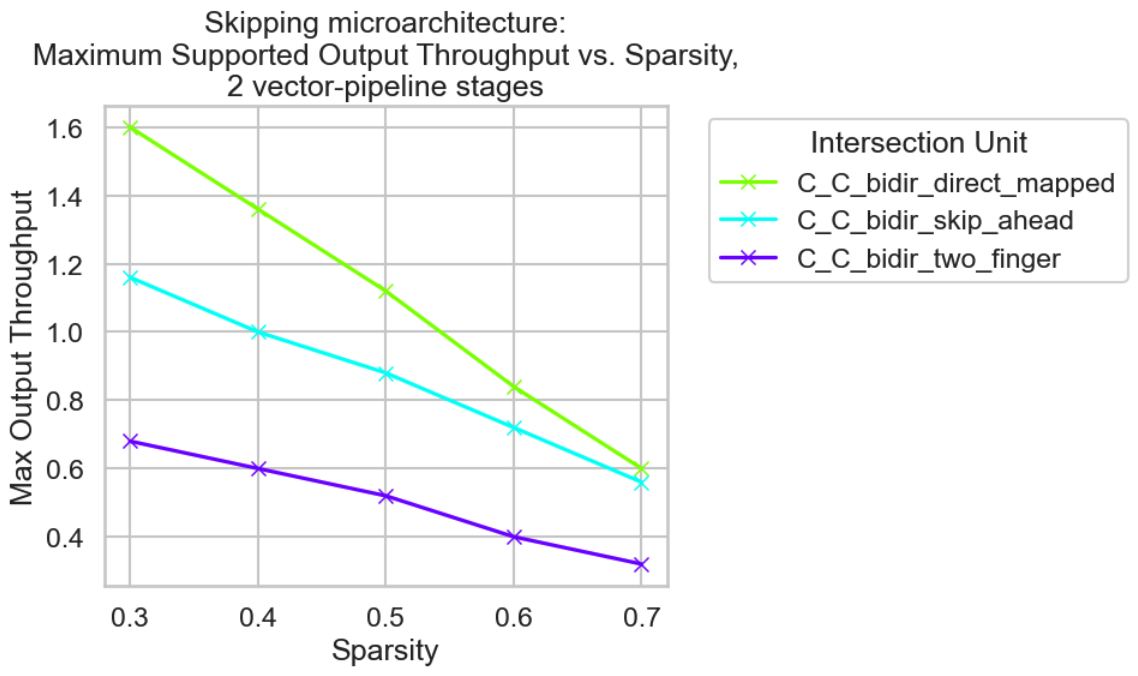
\includegraphics[width=\textwidth]{figures/skip_uarch_pipe_2.png}
\caption{Analysis of intersection unit transfer relations: peak match throughput vs operand sparsity, for intersection units units with two pipeline stages.}
\label{fig:skip_uarch_pipe_2}
\end{figure}

\begin{figure}[H]
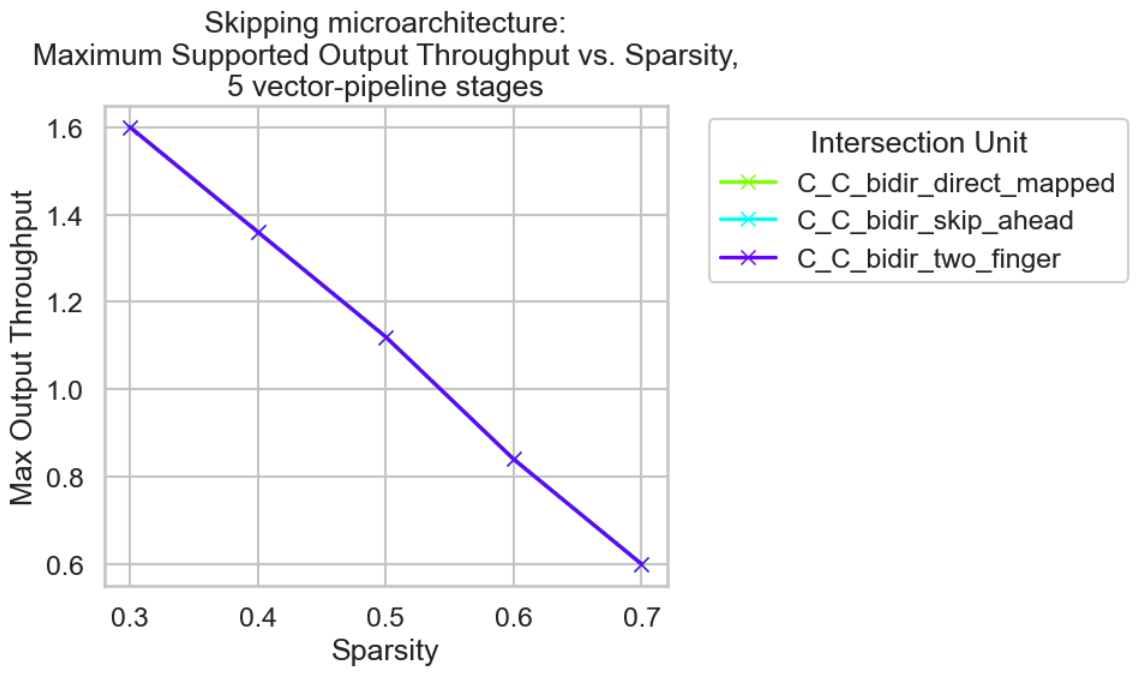
\includegraphics[width=\textwidth]{figures/skip_uarch_pipe_5.png}
\caption{Analysis of intersection unit transfer relations: peak match throughput vs operand sparsity, for intersection units units with five pipeline stages.}
\label{fig:skip_uarch_pipe_5}
\end{figure}

Figures~\ref{fig:skip_uarch_pipe_2} and~\ref{fig:skip_uarch_pipe_5} compare the throughput at the output of the pgen1 units, to the sparsity of the intersection unit input fiber operands, compared between all three intersection unit types for a dense fiber rank size of 16 and a degree-of-vectorization of 4. Figure~\ref{fig:skip_uarch_pipe_2} considers intersection units with 2 pipeline stages while Figure~\ref{fig:skip_uarch_pipe_5} considers intersection units with 5 pipeline stages. 

Note that the relationship between max throughput and sparsity is derived from the transfer relation model that was developed in Section~\ref{sec:c_c_isect_modeling}.

It is clear that pipelining is key to supporting high-throughput intersection, which in turn is critical in a SIMD scenario. It is worth noting that in the scenario shown (vectorization 4, rank size 16), none of these intersection units could supply 2 matches/cycle to support a SIMD 2 arithmetic unit; the max is 1.6 matches/cycle regardless of pipelining. More detailed analysis of the peak matches/cycle throughput supported by each intersection unit variety is provided in Appendix~\ref{appendix:app_intersection_modeling}.

In Figure~\ref{fig:skip_uarch_pipe_2}, direct-mapped intersection attains the highest throughput, followed by skip-ahead intersection unit; this makes sense since direct-mapped intersection has 100\% pipeline efficiency and skip-ahead intersection unit has optimizations to increase pipeline efficiency. This also shows that with 2 pipeline stages, the intersection unit is \textit{efficiency-limited} i.e. limited by how efficient the choice of intersection unit is when it comes to maximizing the number of matches found by a pipeline stage per cycle.

In contrast, in Figure~\ref{fig:skip_uarch_pipe_5}, all intersection units are capable of attaining the same throughput with 5 pipeline stages; this shows that with enough pipeline stages, the intersection unit is \textit{input-rate-limited}, i.e. it is not possible to output more intersections per cycle without changing fiber sparsity, dense rank size, or input vectorization of the intersection unit. Being input-rate-limited is broadly speaking a ``good'' thing, since it means that the particular type of intersection unit we chose is not slowing down the design. We can further observe that while two-finger and skip-ahead intersection unit required multiple pipeline stages in order to be input-rate-limited, direct-mapped intersection unit is already input-rate-limited in Figure~\ref{fig:skip_uarch_pipe_2}. This is because by design, direct-mapped intersection finds all matches in a single cycle, and thus requires only one pipeline stage.

\begin{figure}[H]
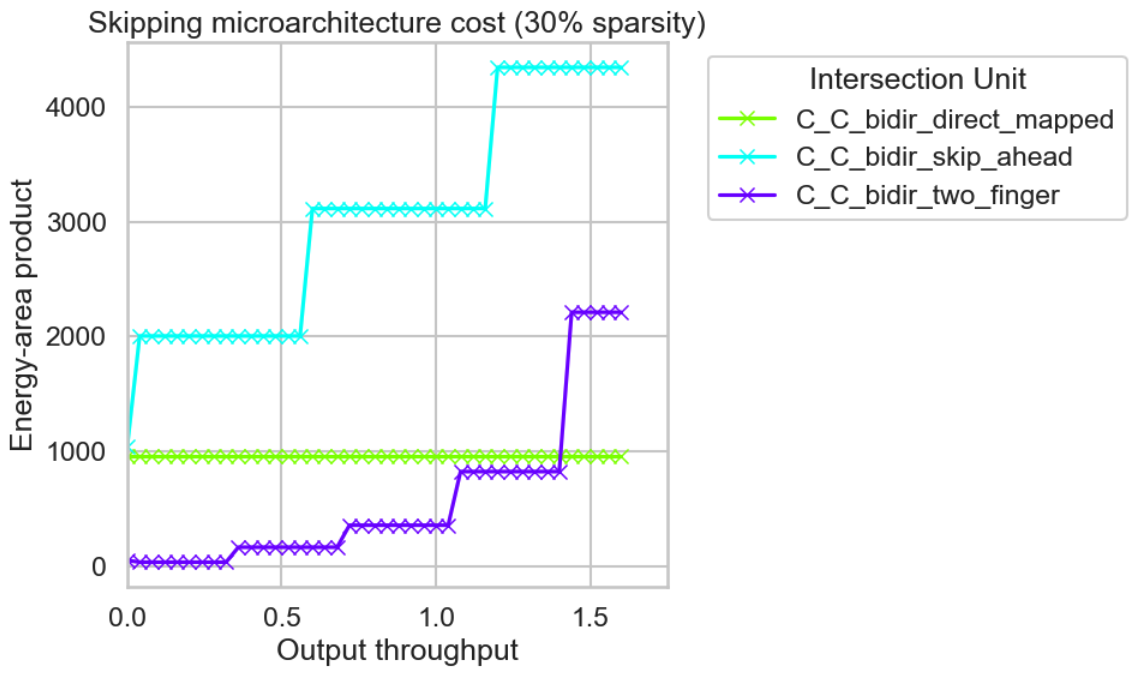
\includegraphics[width=\textwidth]{figures/skip_uarch_sparsity_30pct.png}
\caption{Comparison of energy-per-action/area product for 30\% sparse operands over a range of output throughput requirements.}
\label{fig:skip_uarch_sparsity_30pct}
\end{figure}

\begin{figure}[H]
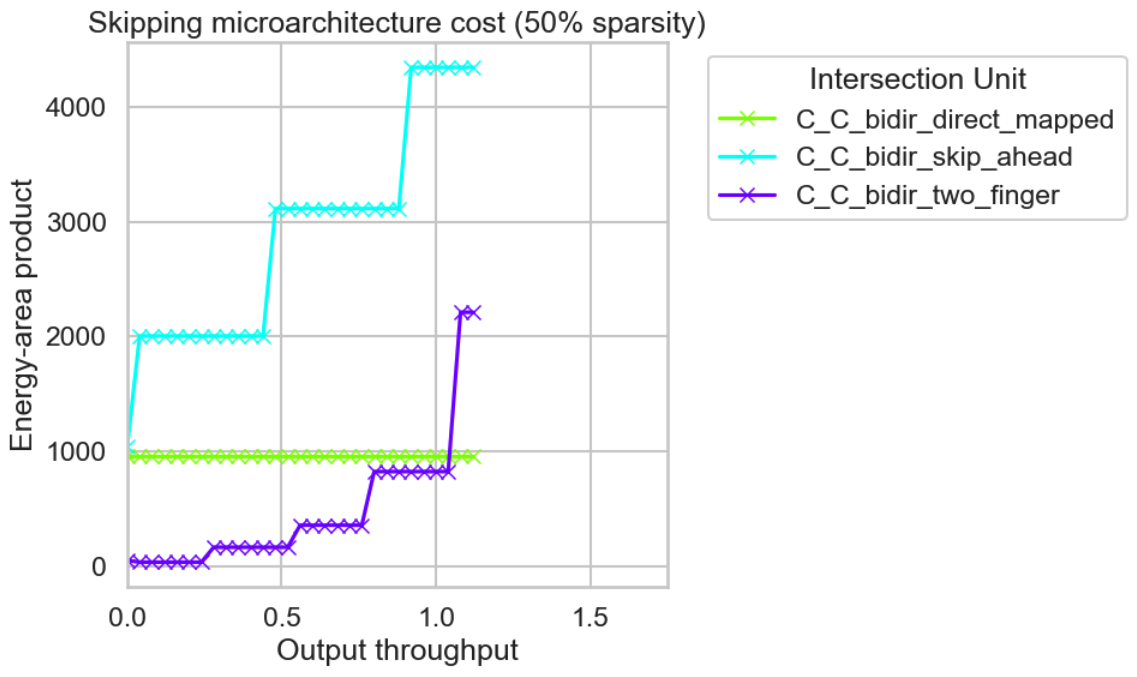
\includegraphics[width=\textwidth]{figures/skip_uarch_sparsity_50pct.png}
\caption{Comparison of energy-per-action/area product for 50\% sparse operands over a range of output throughput requirements..}
\label{fig:skip_uarch_sparsity_50pct}
\end{figure}

\begin{figure}[H]
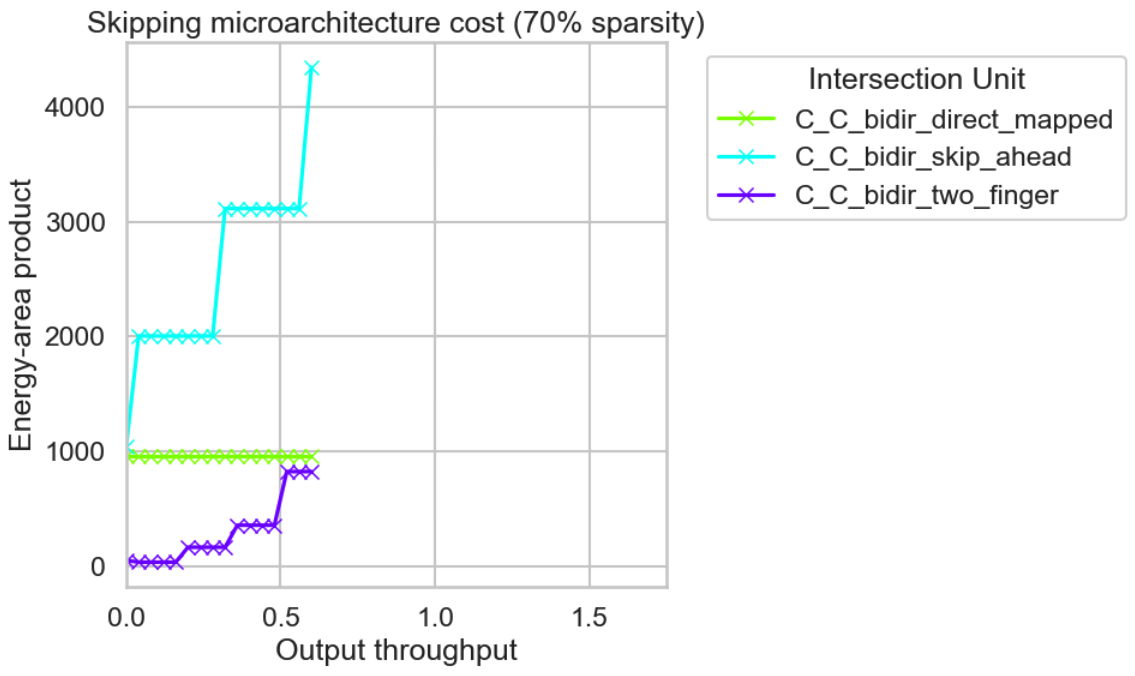
\includegraphics[width=\textwidth]{figures/skip_uarch_sparsity_70pct.png}
\caption{Comparison of energy-per-action/area product for 70\% sparse operands over a range of output throughput requirements..}
\label{fig:skip_uarch_sparsity_70pct}
\end{figure}

Figures~\ref{fig:skip_uarch_sparsity_30pct}, 
~\ref{fig:skip_uarch_sparsity_50pct}, and~\ref{fig:skip_uarch_sparsity_70pct} show how the skipping microarchitecture energy-per-action/area product scales with the output throughput requirement, for each type of intersection unit and for three different sparsity levels. In these figures, the number of pipeline stages is being optimized automatically during scale inference, in order to supply the required throughput. If an intersection unit is not able to supply the requisite throughput with any number of pipeline stages, then the corresponding curve will not have an energy-per-action/area product value associated with that throughput value.

These results suggest that in a SIMD 2 arithmetic scenario, the direct-mapped intersection unit would be a strong candidate for meeting throughput requirement while keeping energy and area low, for the following reasons:

\begin{itemize}
    \item For all sparsities shown, direct-mapped intersection unit has superior energy-per-action/area product \textit{at the highest supported output throughput.}
    \item As shown in Figure~\ref{fig:skip_uarch_pipe_2} Figure~\ref{fig:skip_uarch_pipe_5}, two-finger and skip-ahead intersection unit are efficiency-limited unless they are provisioned with multiple pipeline stages; as shown in Figures~\ref{fig:skip_uarch_sparsity_30pct},~\ref{fig:skip_uarch_sparsity_50pct}, and~\ref{fig:skip_uarch_sparsity_70pct}, this means that the energy-per-action/area product of these intersection units increases substantially with the output throughput design-point. In contrast, direct-mapped intersection unit requires only one pipeline stage regardless of throughput, and thus has uniform energy-per-action and area as the throughput requirement is scaled.
\end{itemize}


Note that in this case study, we are considering intersection units with vector pipelines; however, owing to an early decision to design microarchitecture models based on \textit{combinational unrolling} (Section~\ref{rtl}), the energy-per-action and area characterization results used here are based on combinational unrolling rather than \textit{pipelining}; this means that energy-per-action/area product values quoted in this section may be over-estimates for intersection units with more than one pipeline stage. This could explain the apparent non-linear scaling of two-finger intersection in Figures~\ref{fig:skip_uarch_sparsity_30pct},~\ref{fig:skip_uarch_sparsity_50pct}, and~\ref{fig:skip_uarch_sparsity_70pct}, as combinationally unrolling has non-linear overheads. 

However, it is likely that using energy-per-action and area characterization results based on pipelining, would not significantly change the outcome, because direct-mapped intersection would still have the best pipeline efficiency. Re-running these experiments with models based on pipelining, rather than combinational unrolling, is left for future work.